\scanpage{98}
% archive sheet number: 97
arbitrary. \mbox{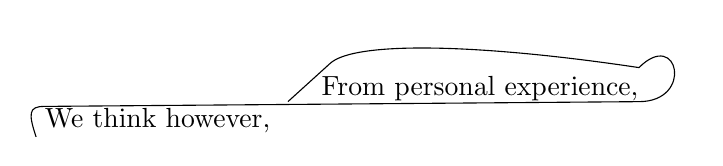
\begin{tikzpicture}[baseline=(base.base)]
\node[inner sep=0] (base) {We think however\deleted{,}};
\node[anchor=south west,inner sep=0,xshift=10em,yshift=.5ex] (added) at (base.north west) {\inserted{From personal experience,}};
\draw ([xshift=-.3em,yshift=-.3ex]base.south west) .. controls +(-.1,.3) and +(-.2,0) .. ([yshift=.1ex]base.north west) -- (added.south east) .. controls +(.7,0) and +(.5,.5) .. ([yshift=.7ex]added.north east) .. controls +(-2,.3) and +(.3,.3) .. ([xshift=.3em,yshift=1ex]added.north west) -- ([xshift=-1.2em]added.south west);
\end{tikzpicture}} that the understanding\deleted{, heuristic although for the moment largely heuristic,} obtained thanks to weight and level arguments, although it is for the moment entirely heuristic, \deleted{is and} may be the source of the discovery of important and unexpected properties for the cohomology of algebraic varieties, \deleted{even if} and that it deserves for this reason not to be disdained. Moreover, in the case of fields of characteristic zero, \deleted{some recent very remar works the magnificent t} the re\rlap{\deleted{\unsure{a|c}}}\handwritten{c}ent and magnificent work of P. DELIGNE on the \mbox{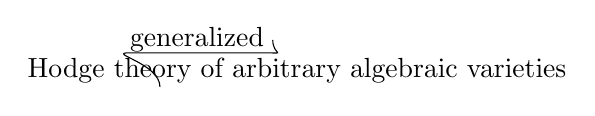
\begin{tikzpicture}[baseline=(base.base)]
\node[inner sep=0] (base) {Hodge theory of arbitrary algebraic varieties};
\node[anchor=south west,inner sep=0,xshift=3.7em,yshift=.4ex] (added) at (base.north west) {\inserted{generalized}};
\draw ([xshift=4.8em,yshift=-.3ex]base.south west) .. controls +(0,.3) and +(-.3,0) .. (added.south west) -- (added.south east) .. controls +(.3,0) and +(0,-.2) .. ([xshift=.3em]added.east);
\end{tikzpicture}} over the field $\underline{C}$ of complex numbers\deleted{,} \mbox{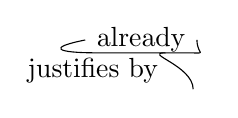
\begin{tikzpicture}[baseline=(base.base)]
\node[inner sep=0] (base) {justifies by};
\node[anchor=south west,inner sep=0,xshift=2.5em,yshift=.4ex] (added) at (base.north west) {\inserted{already}};
\draw ([xshift=-.4em]added.west) .. controls +(-.5,-.1) and +(-.5,0) .. (added.south west) -- (added.south east) .. controls +(.3,0) and +(0,-.2) .. ([xshift=.4em]added.east);
\draw ([xshift=6em,yshift=-.5ex]base.south west) .. controls +(0,.3) and +(-.3,0) .. ([xshift=2.5em]added.south west);
\end{tikzpicture}} transcendental means the ``yoga'' of weights and levels in the framework of De Rham cohomology\handwritten{\unsure{,}} (while opening entirely new paths to the cohomological theory \mbox{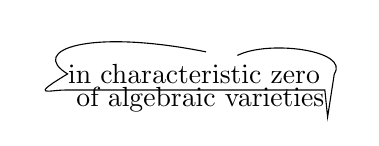
\begin{tikzpicture}[baseline=(base.base)]
\node[inner sep=0] (base) {of algebraic varieties};
\node[anchor=south west,inner sep=0,xshift=-.3em,yshift=.2ex] (added) at (base.north west) {\inserted{in characteristic zero}};
\draw ([xshift=5em,yshift=1ex]added.north west) .. controls +(-1.5,.3) and +(-.5,.3) .. (added.west) .. controls +(-.5,-.3) and +(-.2,0) .. ([xshift=-.4em,yshift=-.3ex]base.north west) -- ([yshift=-.3ex]base.north east) -- ([xshift=.1em,yshift=-.4ex]base.south east) -- ([xshift=.5em]added.east) .. controls +(.2,.3) and +(.4,.2) .. ([xshift=-3em,yshift=.7ex]added.north east);
\end{tikzpicture}}). It \mbox{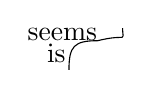
\begin{tikzpicture}[baseline=(old.base)]
\node[inner sep=0] (old) {\deleted{is}};
\node[anchor=south west,inner sep=0,xshift=-.7em,yshift=.2ex] (added) at (old.north west) {\inserted{seems}};
\draw ([xshift=.1em,yshift=-.6ex]old.south east) .. controls +(0,.3) and +(-.3,0) .. (added.south east) .. controls +(.4,.1) and +(0,-.2) .. ([xshift=.9em,yshift=.5ex]added.east);
\end{tikzpicture}} probable on the other hand that for the case of \deleted{To conclude this introduction} alg\rlap{\deleted{b}}\handwritten{e}\rlap{\deleted{\unsure{é|b}}}\handwritten{b}\rlap{\deleted{\unsure{u|r}}}\handwritten{ra}ic\deleted{p} varieties over fields of nonzero characteristic, a justification of this same yoga must await the \mbox{
\begin{tikzpicture}[baseline=(old.base)]
\node[inner sep=0] (old) {\deleted{resolution}};
\node[anchor=south west,inner sep=0,yshift=.1ex] at (old.north west) {\inserted{proof}};
\end{tikzpicture}} of the Weil conjectures (or better, of the ``standard conjectures'' of \handwritten{[\quad]}).

To \deleted{point out c} conclude this introduction, let us point out that the filtrations by weights and levels of the $\handwritten{\ell}$-adic cohomology spaces, for variable $\handwritten{\ell}$, are certainly relat\rlap{\handwritten{e}}\deleted{\unsure{s}}\handwritten{d} to one another in the usual way, \mbox{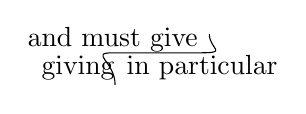
\begin{tikzpicture}[baseline=(old.base)]
\node[inner sep=0] (old) {\deleted{giving}};
\node[anchor=base west,inner sep=0,xshift=.4em] (base) at (old.base east) {in particular};
\node[anchor=south west,inner sep=0,xshift=-.5em,yshift=.2ex] (added) at (old.north west) {\inserted{and must give}};
\draw ([yshift=-.4ex]old.south east) .. controls +(0,.3) and +(-.3,0) .. (added.south) -- (added.south east) .. controls +(.4,0) and +(0,-.2) .. ([xshift=.4em,yshift=.5ex]added.east);
\end{tikzpicture}} vector spaces over $\underline{Q}_{\handwritten{\ell}}$ \rlap{\deleted{e}}\handwritten{w}hose \deleted{ran} rank is independent of $\handwritten{\ell}$. In terms of the conjectural theory of motives (dependent among other things on the ``standard conjectures'' already mentioned), this should be expressed by the fact that the weight \mbox{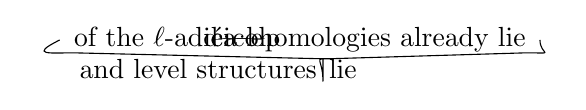
\begin{tikzpicture}[baseline=(base.base)]
\node[inner sep=0] (base) {and level structures};
\node[anchor=base west,inner sep=0,xshift=.4em] (old) at (base.base east) {\deleted{lie}};
\node[anchor=south west,inner sep=0,xshift=-.2em,yshift=.5ex] (added) at (base.north west) {\inserted{of the $\handwritten{\ell}$-ad\rlap{\deleted{\unsure{d|l}}}\handwritten{i}\rlap{\deleted{\unsure{é|e}}}\handwritten{c}\rlap{\deleted{i}}\handwritten{}\rlap{\deleted{\unsure{a|p}}}\handwritten{} cohomologies already lie}};
\draw ([xshift=-.5em]added.west) .. controls +(-.4,-.2) and +(-.3,0) .. (added.south west) -- ([xshift=.2em]base.north east) -- ([xshift=.2em,yshift=-.2ex]base.south east) .. controls +(0,.3) and +(-.2,0) .. (old.north west) -- (added.south east) .. controls +(.4,0) and +(0,-.2) .. ([xshift=.5em]added.east);
\end{tikzpicture}} at the level of \deleted{\unsure{motives|motives} already,} \uline{motivic} \deleted{of the} \uline{cohomology}, \mbox{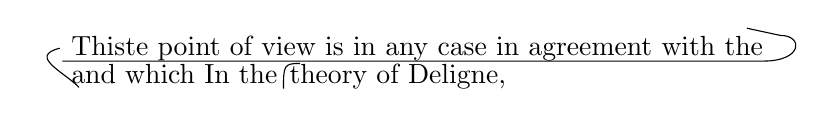
\begin{tikzpicture}[baseline=(old.base)]
\node[inner sep=0] (old) {\deleted{and which In the}};
\node[anchor=base west,inner sep=0,xshift=.4em] (base) at (old.base east) {theory of Deligne,};
\node[anchor=south west,inner sep=0,yshift=.2ex] (added) at (old.north west) {\inserted{This\deleted{te} point of view is in any case in agreement with the}};
\draw ([xshift=-.4em]added.west) .. controls +(-.4,-.1) and +(-.2,.2) .. ([xshift=.3em,yshift=-.3ex]old.south west);
\draw ([xshift=-.3em]added.south west) -- (added.south east) .. controls +(.5,0) and +(.3,0) .. ([xshift=.6em]added.north east) -- ([xshift=-.6em,yshift=.6ex]added.north east);
\draw ([xshift=.2em,yshift=-.4ex]old.south east) .. controls +(0,.3) and +(-.2,0) .. ([xshift=.8em]old.north east);
\end{tikzpicture}} \deleted{\unsure{for}} since his ``weight filtration'' of De Rham cohomology comes from a filtration of cohomology with \uline{rational} coefficients\handwritten{.}\deleted{(and not only}
